\chapter{ANALYSIS}
\label{ANALYSIS}

\section{Analysis}
\label{Analysis}
Mineral aerosol represents one of the largest mass fractions of the global aerosol. It consists of windblown soil and is produced mainly in the arid areas of our planet, in particular in the great deserts. Its annual production rate is estimated to be in the order of 200 to 5000 Tg. The smaller size fraction (< 20 $\mu$m) may be transported over long distances  of up to 5000 km. Mineral aerosol has been considered a nonreactive, hydrophobic surface . Nevertheless, its impact on the atmospheric radiation budget and on the concentration of cloud condensation nuclei (CCN) have been discussed. Recently, its possible role as a surface for heterogeneous reactions has been taken into account.

\subsection{Pedestal\index{Pedestal} Analysis}
\label{Pedestal Analysis}

The main detectors and luminosity monitors are normalized to the charge monitors so it is important that neither have any evidence of helicity correlated pedestal differences. All the charge monitors shows no signs of helicity correlated pedestals.

\subsection{Helicity Correlated Pedestal Signal Pickup}
\label{Helicity Correlated Pedestal Signal Pickup}
The helicity correlated pedestal difference mean from $HelTree$ represent the pickup by a device.

\begin{singlespace}
\begin{figure}[h]
	\centering
%	\begin{center}
	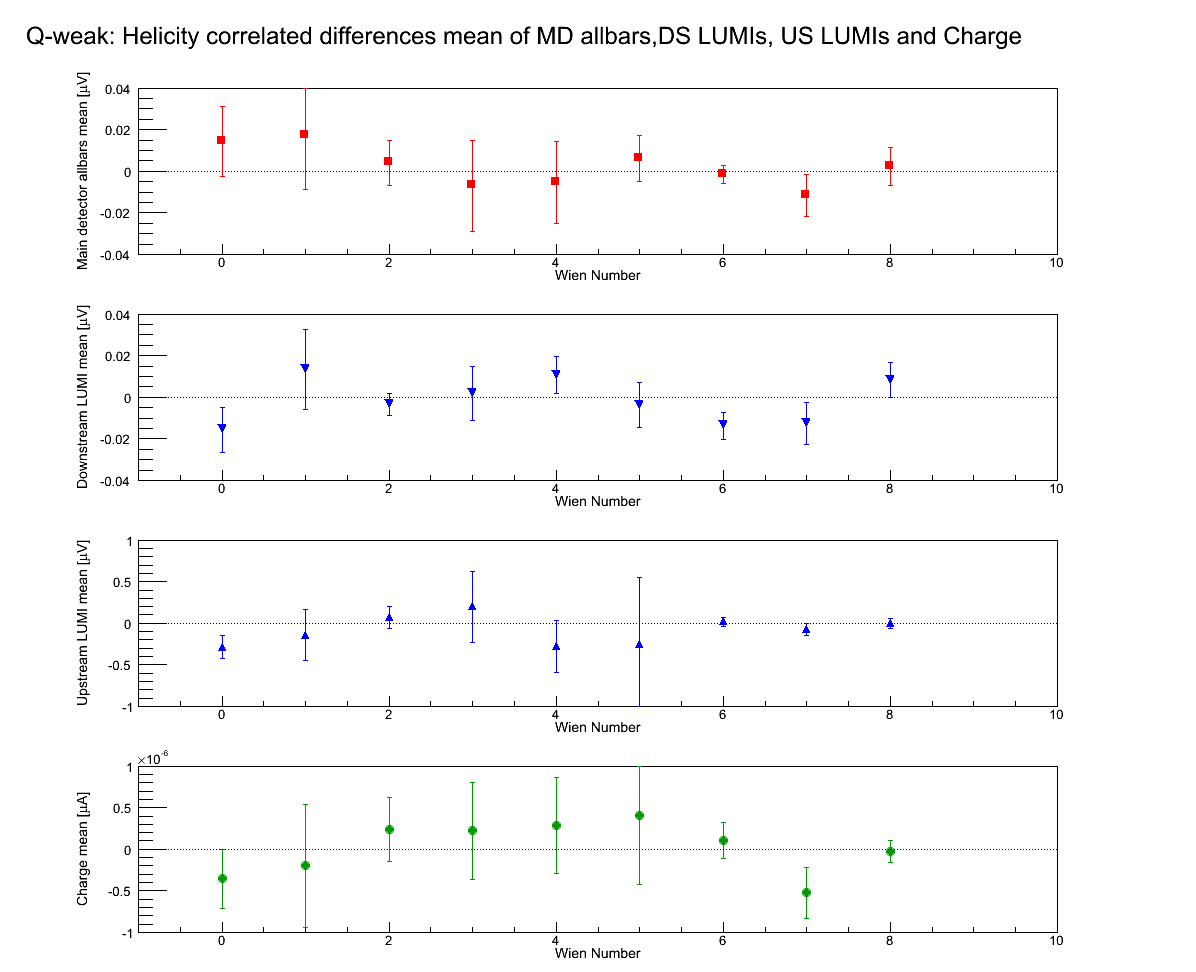
\includegraphics[width=15.0cm]{figures/final_sum_combined_ped_plot}
%	\end{center}
	\caption
	[Final result summary.]
	{Final result summary. Panel 1 shows the helecity correlated main detector all bars. Panel 2 shows the helecity correlated downstream luminosity monitors. Panel 3 shows the helecity correlated upstream luminosity monitors. Panel 4 shows the helecity correlated charge monitors.}
	\label{fig:final_sum_combined_ped_plot}
\end{figure}
\end{singlespace}

\begin{singlespace}
\begin{figure}[h]
	\centering
%	\begin{center}
	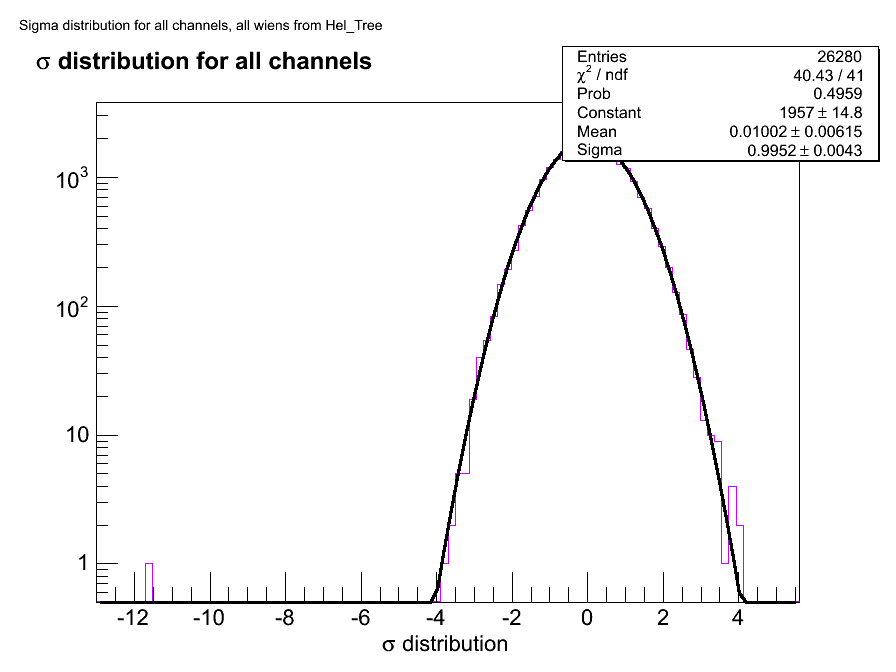
\includegraphics[width=15.0cm]{FIGURES/HelCorDiffSigmaDistribution}
%	\end{center}
	\caption
	[Final result using pull plot.]
	{Final result using pull plot. Sigma  distribution for all the channel and wien.}
	\label{fig:HelCorDiffSigmaDistribution}
\end{figure}
\end{singlespace}

Helicity correlated pickup during Q-weak running was consistent with zero for all channels, with a sensitivity at the $\pm$ 1 ppb level for most channels. 

The distribution of $\sigma$ is Gaussian and mean is zero for each channel and run. The few $\sigma$ from zero pickup for different detectors are within the statistical fluctuation of the $\sigma$  distribution.

No evidence of helicity correlated pickup. 

\subsection{Helicity Correlated Pedestal Sensitivities}
\label{Helicity Correlated Pedestal Sensitivities}
The helicity correlated pedestal difference width from $HelTree$ represent the sensitivity of a device with helicity.

Width of helicity correlated differences are measure of electronic noise level for our detectors with low frequency rejection.

MDs, DSLumis noise levels acceptable and reasonably stable.

USLumi electronic noise could have limited that detectorÕs resolution near end of Run 1, but improved in Run 2 after repairs. 



\subsection{Mean of Pedestal Subtracted Signal from Mps$\_$Tree}
\label{Mean of Pedestal Subtracted Signal from $MpsTree$}
The mean of pedestal subtracted signal from $MpsTree$ represent the relative change in pedestal signal compared to last pedestal.

A wrong pedestal for a detector can cause nonlinearity.

MD pedestal is good to a few mV. Resulting nonlinearity would 
	be << 0.1$\%$ for 6V signals. Would still be < 1$\%$ even allowing for smaller yields from Aluminum or N-to-Delta. 
DSLumi pedestal off by at most 34 mV. Resulting nonlinearity would be < 1$\%$ assuming 6V signals. To support Aluminum running, etc., pedestal subtraction should be improved in Wiens 2, 9, 10. 
USLumi pedestal off by 100-150 mV in Wiens 7,8. Resulting nonlinearity would be several percent assuming 6V signals. To support Aluminum running, etc., must be improved.  




\subsection{Width of Pedestal Subtracted Signal from $MpsTree$}
\label{Width of Pedestal Subtracted Signal from $MpsTree$}
The width of pedestal subtracted signal from $MpsTree$ represent the detector resolution.